\section{極限}\label{chap-8-limit}

\begin{define}[極限]\label{def-limit}
  ある圏$\cat{C},\cat{D}$と関手$\functor{F}{C}{D}$に対する極限$(\lim F, \nu)$を以下のように構成する。
  \begin{quote}
    \begin{mydescription}
      \item[錐] 錐と呼ばれる組$(X,\mu)$を以下のように構成する。
      圏$\cat{D}$の対象である$X$と、
      圏$\cat{C}$の任意の対象$C$に対して$\mor{\mu_C}{X}{FC}$なる射が存在し、圏$\cat{C}$の任意の射$\mor{f}{A}{B}$に対して$\mu_B=Ff\circ\mu_A$が成り立つ。
      \begin{center}
        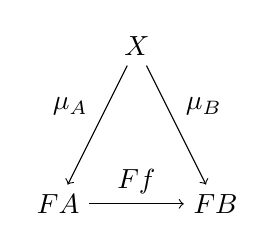
\begin{tikzpicture}[auto]
          \node (limf) at (0, 2) {$X$};
          \node (fa) at (-1, 0) {$FA$};
          \node (fb) at (1, 0) {$FB$};
          \draw[->] (limf) to node[swap]{$\mu_A$}(fa);
          \draw[->] (limf) to node{$\mu_B$}(fb);
          \draw[->] (fa) to node{$Ff$}(fb);
        \end{tikzpicture}
      \end{center}
      
      またこの対象ごとの射は自然変換で表せる。$\mor{\mu}{\Delta X}{F}$とすると、対象$C$の成分は$\mor{\mu_C}{X}{FC}$であり、等式$\mu_B=Ff\circ\mu_A$は自然変換の自然性にあたる。
      \begin{center}
        \begin{tikzpicture}[auto]
          \node (catc) at (-4, 3) {$\cat{C}$};
          \node (a) at (-5, 1) {$A$};
          \node (b) at (-3, 1) {$B$};
          \draw[->] (a) to node{$f$}(b);

          \node (catd) at (0, 3) {$\cat{D}$};
          \node (limf) at (0, 2) {$X$};
          \node (fa) at (-1, 0) {$FA$};
          \node (fb) at (1, 0) {$FB$};
          \draw[->] (limf) to node[swap]{$\mu_A$}(fa);
          \draw[->] (limf) to node{$\mu_B$}(fb);
          \draw[->] (fa) to node{$Ff$}(fb);

          \draw[->,bend left = 20] (catc) to node (funcf){$\varDelta X$}(catd);
          \draw[->,bend right = 20] (catc) to node (funcg)[swap]{$F$}(catd);
          \draw[double,double equal sign distance,-implies,shorten >=5pt,shorten <=5pt] (funcf) -- node[label=right:$\mu$] {} (funcg);
        \end{tikzpicture}
      \end{center}
      \item[普遍性] ある錐$(\lim F, \tau)$が極限であるとは、他の錐$(X,\mu)$に対して、$\tau_C = \nu_C\circ h$が成り立つような$\mor{h}{X}{\lim F}$が一意に存在する。すなわち自然変換$\mu$は$\tau$によって射$h$へと分解される。
      \begin{center}
        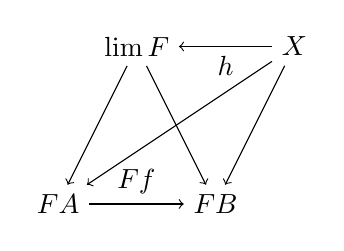
\begin{tikzpicture}[auto]
          \node (limf) at (0, 2) {$\lim F$};
          \node (x) at (2, 2) {$X$};

          \node (fa) at (-1, 0) {$FA$};
          \node (fb) at (1, 0) {$FB$};
          \draw[->] (limf) to node{}(fa);
          \draw[->] (limf) to node{}(fb);
          \draw[->] (x) to node[swap]{}(fa);
          \draw[->] (x) to node{}(fb);
          \draw[->] (fa) to node{$Ff$}(fb);
          \draw[->] (x) to node{$h$}(limf);
        \end{tikzpicture}
        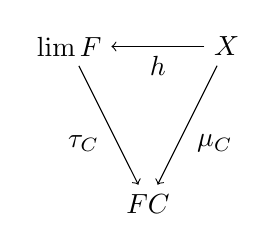
\begin{tikzpicture}[auto]
          \node (limf) at (0, 2) {$\lim F$};
          \node (x) at (2, 2) {$X$};

          \node (fa) at (1, 0) {$FC$};
          \draw[->] (limf) to node[swap]{$\tau_C$}(fa);
          \draw[->] (x) to node{$\mu_C$}(fa);
          \draw[->] (x) to node{$h$}(limf);
        \end{tikzpicture}
      \end{center}
    \end{mydescription}
  \end{quote}
\end{define}
\begin{prop}[極限の一意性]\label{prop-uniqueness-of-limits}
  関手$F$に対する極限$(\lim F, \nu)$が存在するとする。同様に$(X, \tau)$も関手$F$に対する極限であるならば、$\lim F\cong X$である。
\end{prop}
\begin{proof}
  積や終対象の一意性と同様に証明する。

  極限の定義から、$\mor{h}{X}{\lim F}$なる射が一意に存在するが、同時に$X$も極限対象であるから$\mor{h^{-1}}{\lim F}{X}$が一意に存在する。この二つの射が同型射になることを示せば良い。

  以下の図式から、$\tau_C =\tau_C h^{-1}\circ h$となる$h^{-1}\circ h$は極限の普遍性によって一意に定まるが、同様に恒等射$\mor{id_{lim F}}{lim F}{lim F}$も$\tau_C =\tau_C \circ id_{lim F}$であるから、一意性より$h^{-1}\circ h=id_{lim F}$となる。

  同様に$h\circ h^{-1} = id_X$も示せるから$\lim F\cong X$である。

  \begin{center}
    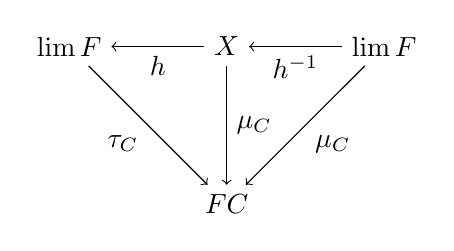
\begin{tikzpicture}[auto]
      \node (limf) at (0, 2) {$\lim F$};
      \node (x) at (2, 2) {$X$};
      \node (limf2) at (4, 2) {$\lim F$};
      \node (fa) at (2, 0) {$FC$};
      \draw[->] (limf) to node[swap]{$\tau_C$}(fa);
      \draw[->] (x) to node{$\mu_C$}(fa);
      \draw[->] (limf2) to node{$\mu_C$}(fa);
      \draw[->] (x) to node{$h$}(limf);
      \draw[->] (limf2) to node{$h^{-1}$}(x);
    \end{tikzpicture}
    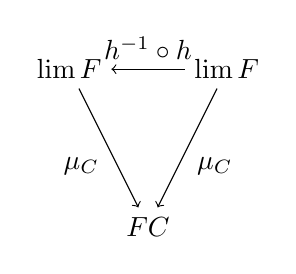
\begin{tikzpicture}[auto]
      \node (limf) at (0, 2) {$\lim F$};
      \node (x) at (2, 2) {$\lim F$};

      \node (fa) at (1, 0) {$FC$};
      \draw[->] (limf) to node[swap]{$\mu_C$}(fa);
      \draw[->] (x) to node{$\mu_C$}(fa);
      \draw[->] (x) to node[swap]{$h^{-1}\circ h$}(limf);
    \end{tikzpicture}
  \end{center}

\end{proof}
\begin{define}[完備]\label{def-completeness}
  圏$\cat{D}$が完備であるとは、任意の関手$\functor{F}{C}{D}$に対して極限$(\lim F, \tau)$を持つことである。
\end{define}
\begin{prop}[極限の関手性]\label{prop-limit-is-functor}
  圏$\cat{D}$が完備であるとする。任意の関手$\functor{F}{C}{D}$に対して極限対象$\lim F$を得る操作は関手である。すなわち$\mor{\lim}{\funccat{C}{D}}{D}$である。
\end{prop}
\begin{proof}
  \begin{quote}~
    \begin{mydescription}
      \item[対象関数] 任意の関手$\functor{F}{C}{D}$に対して対象関数を$\lim(F) = \lim F$と定義する。
      \item[射関数] 
      任意の自然変換$\nat{\alpha}{F}{G}$に対して、射関数によって写された射$\lim \alpha$を考える。

      関手$F,G$による極限を$(\lim F, \tau),(\lim G, \nu)$とすると、極限$(\lim G, \nu)$の普遍性より$\mor{h}{\lim F}{\lim G}$への射が一意に存在する。
      \begin{center}
        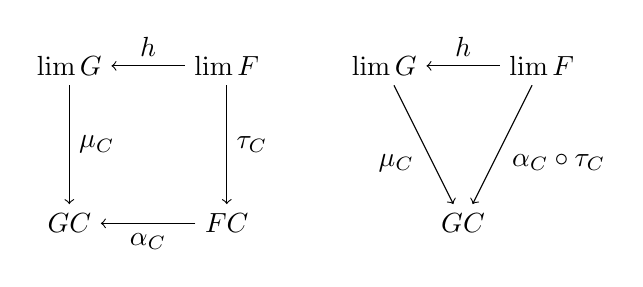
\begin{tikzpicture}[auto]
          \node (limf) at (2, 0) {$\lim F$};
          \node (limg) at (0, 0) {$\lim G$};

          \node (fa) at (2, -2) {$FC$};
          \node (ga) at (0, -2) {$GC$};
          \draw[->] (limf) to node{$\tau_C$}(fa);
          \draw[->] (limg) to node{$\mu_C$}(ga);
          \draw[->] (fa) to node{$\alpha_C$}(ga);
          \draw[->] (limf) to node[swap]{$h$}(limg);

          \node (limf) at (4, 0) {$\lim G$};
          \node (x) at (6, 0) {$\lim F$};
    
          \node (fa) at (5, -2) {$GC$};
          \draw[->] (limf) to node[swap]{$\mu_C$}(fa);
          \draw[->] (x) to node{$\alpha_C\circ \tau_C$}(fa);
          \draw[->] (x) to node[swap]{$h$}(limf);
        \end{tikzpicture}
        \begin{tikzpicture}[auto]

        \end{tikzpicture}
      \end{center}
      この射を$\lim\alpha$とし、$\lim(\alpha)=\lim\alpha$とする。
      \item[恒等射の保存] $\lim(ID_F)=id_{\lim F}$を示せば良い。$\tau_C\circ id_{\lim F} = \tau_C$であるが、極限の普遍性よりこのような射は一意にさだまる。よって$h=id_{\lim F}$であり恒等射を保つ。
      \begin{center}
        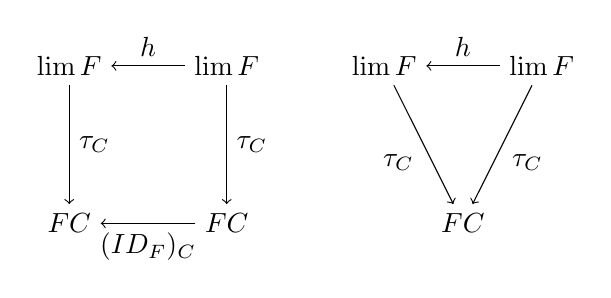
\begin{tikzpicture}[auto]
          \node (limf) at (2, 0) {$\lim F$};
          \node (limg) at (0, 0) {$\lim F$};

          \node (fa) at (2, -2) {$FC$};
          \node (ga) at (0, -2) {$FC$};
          \draw[->] (limf) to node{$\tau_C$}(fa);
          \draw[->] (limg) to node{$\tau_C$}(ga);
          \draw[->] (fa) to node{$(ID_F)_C$}(ga);
          \draw[->] (limf) to node[swap]{$h$}(limg);

          \node (limf) at (4, 0) {$\lim F$};
          \node (x) at (6, 0) {$\lim F$};
    
          \node (fa) at (5, -2) {$FC$};
          \draw[->] (limf) to node[swap]{$\tau_C$}(fa);
          \draw[->] (x) to node{$\tau_C$}(fa);
          \draw[->] (x) to node[swap]{$h$}(limf);
        \end{tikzpicture}
      \end{center}
      \item[射の合成の保存] $\lim (\beta\cdot\alpha)=\lim \beta\circ \lim\alpha$を示せば良い。極限$(\lim F,\tau),(\lim G,\nu),(\lim H,\mu)$と自然変換$\nat{\alpha}{F}{G},\ \nat{\beta}{G}{H}$に対して、
      \[(\beta\cdot\alpha)_C\circ\tau_C=\mu_C\circ\lim\beta\circ\lim\alpha \]が成り立つが、射関数の定義と射の一意性により$\lim (\beta\cdot\alpha)=\lim\beta\circ\lim\alpha$が成り立つ。
      \begin{center}
        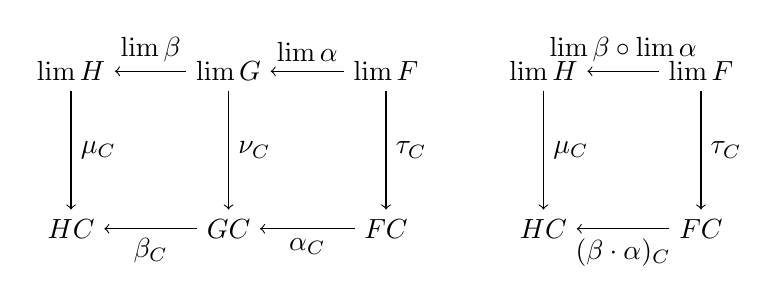
\begin{tikzpicture}[auto]
          \node (limf) at (2, 0) {$\lim F$};
          \node (limg) at (0, 0) {$\lim G$};
          \node (limh) at (-2, 0) {$\lim H$};

          \node (fa) at (2, -2) {$FC$};
          \node (ga) at (0, -2) {$GC$};
          \node (ha) at (-2, -2) {$HC$};

          \draw[->] (limf) to node{$\tau_C$}(fa);
          \draw[->] (limg) to node{$\nu_C$}(ga);
          \draw[->] (limh) to node{$\mu_C$}(ha);

          \draw[->] (fa) to node{$\alpha_C$}(ga);
          \draw[->] (ga) to node{$\beta_C$}(ha);

          \draw[->] (limf) to node[swap]{$\lim \alpha$}(limg);
          \draw[->] (limg) to node[swap]{$\lim \beta$}(limh);


          \node (limf) at (6, 0) {$\lim F$};
          \node (limg) at (4, 0) {$\lim H$};

          \node (fa) at (6, -2) {$FC$};
          \node (ga) at (4, -2) {$HC$};
          \draw[->] (limf) to node{$\tau_C$}(fa);
          \draw[->] (limg) to node{$\mu_C$}(ga);
          \draw[->] (fa) to node{$(\beta\cdot\alpha)_C$}(ga);
          \draw[->] (limf) to node[swap]{$\lim\beta\circ\lim\alpha$}(limg);
        \end{tikzpicture}
      \end{center}
    \end{mydescription}
  \end{quote}
\end{proof}
%\begin{prop}[射集合による定義]\label{prop-def-limit-by-arrowset}
%  $\arset{D}{X}{\lim F}\cong\arset{\funccat{C}{D}}{\varDelta X}{F}$で$X$と$F$に対して自然$\iff \lim$は極限を取る関手
%\end{prop}
\begin{prop}[共変Hom関手の極限の保存]
  $\arset{D}{X}{\lim F}\cong\lim\arset{C}{X}{F-}$であり$X$に対して自然
\end{prop}
\begin{proof}
  共変Hom関手の積の保存と同様に示す。つまり$\arset{D}{X}{\lim F}$が関手$\functor{\arset{C}{X}{F-}}{C}{Set}$の極限であることを示せば良い。
  \begin{center}
    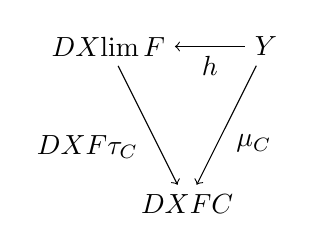
\begin{tikzpicture}[auto]
      \node (limf) at (0, 2) {$\arset{D}{X}{\lim F}$};
      \node (x) at (2, 2) {$Y$};

      \node (fa) at (1, 0) {$\arset{D}{X}{FC}$};
      \draw[->] (limf) to node[swap]{$\arset{D}{X}{F\tau_C}$}(fa);
      \draw[->] (x) to node{$\mu_C$}(fa);
      \draw[->] (x) to node{$h$}(limf);
    \end{tikzpicture}
  \end{center}
  また$\arset{D}{X}{F\tau_C}$は、関手$\arset{D}{X}{F-}$と自然変換$\tau$の水平合成で得られる自然変換であるため、自然性を保つ。


  $Y$を$1$に制限する。
  \begin{center}
    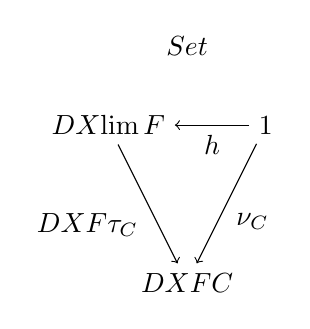
\begin{tikzpicture}[auto]
      \node (x) at (1, 3) {$\cat{Set}$};

      \node (limf) at (0, 2) {$\arset{D}{X}{\lim F}$};
      \node (x) at (2, 2) {$1$};

      \node (fa) at (1, 0) {$\arset{D}{X}{FC}$};
      \draw[->] (limf) to node[swap]{$\arset{D}{X}{F\tau_C}$}(fa);
      \draw[->] (x) to node{$\nu_C$}(fa);
      \draw[->] (x) to node{$h$}(limf);
    \end{tikzpicture}
    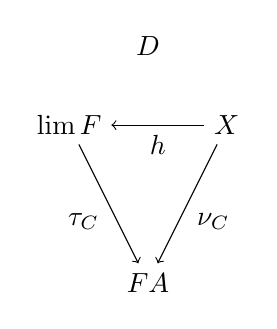
\begin{tikzpicture}[auto]
      \node (x) at (1, 3) {$\cat{D}$};

      \node (limf) at (0, 2) {$\lim F$};
      \node (x) at (2, 2) {$X$};
      \node (fa) at (1, 0) {$FA$};
      \draw[->] (limf) to node[swap]{$\tau_C$}(fa);
      \draw[->] (x) to node{$\nu_C$}(fa);
      \draw[->] (x) to node{$h$}(limf);
    \end{tikzpicture}
  \end{center}

  圏$\cat{C}$において$\tau$が自然変換であるのは分かるが、$\nu$が自然変換であることを念の為確かめる。
  \begin{center}
    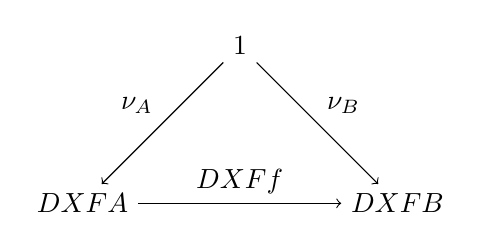
\begin{tikzpicture}[auto]
      \node (limf) at (0, 2) {$1$};
      \node (fa) at (-2, 0) {$\arset{D}{X}{FA}$};
      \node (fb) at (2, 0) {$\arset{D}{X}{FB}$};
      \draw[->] (limf) to node[swap]{$\nu_A$}(fa);
      \draw[->] (limf) to node{$\nu_B$}(fb);
      \draw[->] (fa) to node{$\arset{D}{X}{Ff}$}(fb);
    \end{tikzpicture}
  \end{center}
\end{proof}
\begin{define}[エンド]\label{def-end}
  ある圏$\cat{C,D}$と、関手$\functor{F}{C^{op}\times C}{D}$に対するエンド$(\displaystyle\int_{c:\cat{C}} F(C,C),\lambda)$を以下のように構成する。
  \begin{quote}
    \begin{mydescription}
      \item[エンド対象]圏$\cat{D}$のある対象$\displaystyle\int_{c:\cat{C}} F(C,C)$
      \item[射影射] 圏$\cat{C}$の任意の対象$X$に対して$\mor{\lambda_C}{\displaystyle\int_{c:\cat{C}} F(C,C)}{F(X,X)}$なる射が存在し、圏$\cat{C}$の任意の射$\mor{f}{A}{B}$に対して$F(A,f)\circ\lambda_A=F(f,B)\circ\lambda_B$が成り立つ。
      \begin{center}
        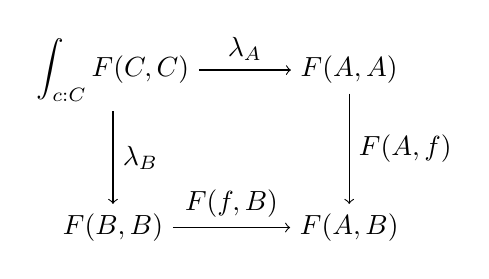
\begin{tikzpicture}[auto]
          \node (FG) at (0, 0) {$\displaystyle\int_{c:\cat{C}} F(C,C)$};
          \node (FAGA) at (3, 0) {$F(A,A)$};
          \node (FBGB) at (0, -2) {$F(B,B)$};
          \node (FAGB) at (3, -2) {$F(A,B)$};
  
          \draw[->] (FG) to node{$\lambda_A$}(FAGA);  
          \draw[->] (FG) to node{$\lambda_B$}(FBGB);
          \draw[->] (FAGA) to node{$F(A,f)$}(FAGB);
          \draw[->] (FBGB) to node{$F(f,B)$}(FAGB);
        \end{tikzpicture}
      \end{center}
      \item[普遍性] $F$に対して同様の条件を満たす$(Y,\mu)$が存在する時、任意の対象$X$において$\mu=\lambda_X\circ h$が成り立つような$\mor{h}{Y}{\displaystyle\int_{c:\cat{C}} F(C,C)}$が一意に存在する。
      \begin{center}
        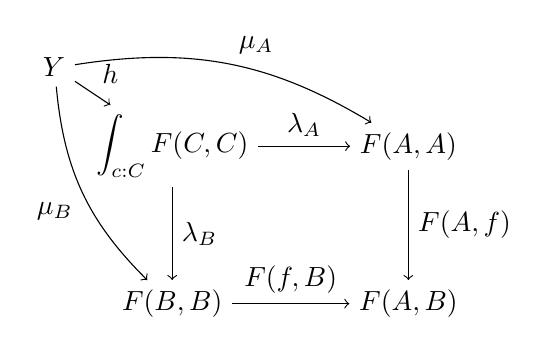
\begin{tikzpicture}[auto]
          \node (FG) at (0, 0) {$\displaystyle\int_{c:\cat{C}} F(C,C)$};
          \node (X) at (-1.5, 1) {$Y$};
          \node (FAGA) at (3, 0) {$F(A,A)$};
          \node (FBGB) at (0, -2) {$F(B,B)$};
          \node (FAGB) at (3, -2) {$F(A,B)$};
  
          \draw[->] (FG) to node{$\lambda_A$}(FAGA);
          \draw[->] (X) to node{$h$}(FG);
  
          \draw[->] (FG) to node{$\lambda_B$}(FBGB);
          \draw[->,bend left = 20] (X) to node{$\mu_A$}(FAGA);
          \draw[->,bend right = 20] (X) to node[swap]{$\mu_B$}(FBGB);
          \draw[->] (FAGA) to node{$F(A,f)$}(FAGB);
          \draw[->] (FBGB) to node{$F(f,B)$}(FAGB);
        \end{tikzpicture}
      \end{center}
    \end{mydescription}
  \end{quote}
\end{define}
エンドの定義から自然変換の射集合は明らかにエンドである。
\begin{prop}
  $\arset{\funccat{C}{D}}{F}{G}=\displaystyle\int_{c:\cat{C}} \arset{D}{FC}{GC}$
\end{prop}